% Options for packages loaded elsewhere
\PassOptionsToPackage{unicode}{hyperref}
\PassOptionsToPackage{hyphens}{url}
%
\documentclass[
]{book}
\usepackage{lmodern}
\usepackage{amssymb,amsmath}
\usepackage{ifxetex,ifluatex}
\ifnum 0\ifxetex 1\fi\ifluatex 1\fi=0 % if pdftex
  \usepackage[T1]{fontenc}
  \usepackage[utf8]{inputenc}
  \usepackage{textcomp} % provide euro and other symbols
\else % if luatex or xetex
  \usepackage{unicode-math}
  \defaultfontfeatures{Scale=MatchLowercase}
  \defaultfontfeatures[\rmfamily]{Ligatures=TeX,Scale=1}
\fi
% Use upquote if available, for straight quotes in verbatim environments
\IfFileExists{upquote.sty}{\usepackage{upquote}}{}
\IfFileExists{microtype.sty}{% use microtype if available
  \usepackage[]{microtype}
  \UseMicrotypeSet[protrusion]{basicmath} % disable protrusion for tt fonts
}{}
\makeatletter
\@ifundefined{KOMAClassName}{% if non-KOMA class
  \IfFileExists{parskip.sty}{%
    \usepackage{parskip}
  }{% else
    \setlength{\parindent}{0pt}
    \setlength{\parskip}{6pt plus 2pt minus 1pt}}
}{% if KOMA class
  \KOMAoptions{parskip=half}}
\makeatother
\usepackage{xcolor}
\IfFileExists{xurl.sty}{\usepackage{xurl}}{} % add URL line breaks if available
\IfFileExists{bookmark.sty}{\usepackage{bookmark}}{\usepackage{hyperref}}
\hypersetup{
  pdftitle={O czym śpiewają Holendrzy?},
  pdfauthor={Jacek Pardyak},
  hidelinks,
  pdfcreator={LaTeX via pandoc}}
\urlstyle{same} % disable monospaced font for URLs
\usepackage{longtable,booktabs}
% Correct order of tables after \paragraph or \subparagraph
\usepackage{etoolbox}
\makeatletter
\patchcmd\longtable{\par}{\if@noskipsec\mbox{}\fi\par}{}{}
\makeatother
% Allow footnotes in longtable head/foot
\IfFileExists{footnotehyper.sty}{\usepackage{footnotehyper}}{\usepackage{footnote}}
\makesavenoteenv{longtable}
\usepackage{graphicx}
\makeatletter
\def\maxwidth{\ifdim\Gin@nat@width>\linewidth\linewidth\else\Gin@nat@width\fi}
\def\maxheight{\ifdim\Gin@nat@height>\textheight\textheight\else\Gin@nat@height\fi}
\makeatother
% Scale images if necessary, so that they will not overflow the page
% margins by default, and it is still possible to overwrite the defaults
% using explicit options in \includegraphics[width, height, ...]{}
\setkeys{Gin}{width=\maxwidth,height=\maxheight,keepaspectratio}
% Set default figure placement to htbp
\makeatletter
\def\fps@figure{htbp}
\makeatother
\setlength{\emergencystretch}{3em} % prevent overfull lines
\providecommand{\tightlist}{%
  \setlength{\itemsep}{0pt}\setlength{\parskip}{0pt}}
\setcounter{secnumdepth}{5}
% new for polish
\usepackage{polski}
\usepackage[polish]{babel}
%\usepackage[utf8]{inputenc}

% ------------
\usepackage{booktabs}
\usepackage{amsthm}
\makeatletter
\def\thm@space@setup{%
  \thm@preskip=8pt plus 2pt minus 4pt
  \thm@postskip=\thm@preskip
}
% ------------
% new for columns
\newenvironment{columns}[1][]{}{}

\newenvironment{column}[1]{\begin{minipage}{#1}\ignorespaces}{%
\end{minipage}
\ifhmode\unskip\fi
\aftergroup\useignorespacesandallpars}

\def\useignorespacesandallpars#1\ignorespaces\fi{%
#1\fi\ignorespacesandallpars}

\makeatletter
\def\ignorespacesandallpars{%
  \@ifnextchar\par
    {\expandafter\ignorespacesandallpars\@gobble}%
    {}%
}
\makeatother
\usepackage[]{natbib}
\bibliographystyle{apalike}

\title{O czym śpiewają Holendrzy?}
\author{Jacek Pardyak}
\date{2020-05-03}

\begin{document}
\maketitle

{
\setcounter{tocdepth}{1}
\tableofcontents
}
\hypertarget{wstux119p}{%
\chapter{Wstęp}\label{wstux119p}}

Wszelkie prawa do tekstów piosenek umieszczonych w tej pracy przysługują ich właścicielom.

Teksty piosenek znajdują się tutaj wyłącznie w celach informacyjnych i edukacyjnych oraz służą do użytku prywatnego.

W przypadku, gdy właściciel praw do konkretnego tekstu nie życzy sobie by się nim posługiwać w tej pracy, uprzejmie proszę o kontakt, a tekst zostanie usunięty.

Wszelkie prawa do tłumaczeń tekstów piosenek umieszczonych w tej pracy przysługują mi, ich autorowi.

W tłumaczeniach staram się utrzymać funkcjonalność orygnialnego tekstu. Jeżeli w przekazie są emocje chcę je również czuć w tłumaczeniu. Chcę przy tym zachować oryginalne słowa, za wyjątkiem gdy w oryginale znajduje się wyrażenie. Wtedy poszukuję podobnego wyrażenia w języku polskim. Nie jest moją intencja dokonwyać adapatacj! piosenek, czyli tworzyć utworóW, które tak samo łatwo da się wyśpiewać nie zważając na oryginalnie użyty słownik.

\hypertarget{top-2000}{%
\chapter{TOP 2000}\label{top-2000}}

\hypertarget{Leef}{%
\section{\texorpdfstring{Leef, \emph{André Hazes jr.}}{Leef, André Hazes jr.}}\label{Leef}}

\begin{column}{0.33\textwidth}

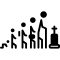
\includegraphics{./images/Leef}

\end{column}

\begin{column}{0.34\textwidth}

~

\end{column}

\begin{column}{0.33\textwidth}

\textbf{Leef} \citep{Leef} {[}\emph{Żyj}{]} to piosenka o życiu i umieraniu. Rozpoczyna się w scenerii podobnej do tej z piosenki \ref{Een-beetje-verliefd} wykonanej przez ojca André Hazes.

\end{column}

\vfill

\begin{column}{0.48\textwidth}

Op een vrijdag in de kroeg ergens in Amsterdam\\
Zat aan de bar met een glas een oude wijze man\\
Hij zei dat die nog maar een paar dagen had\\
Dus pak het leven, pak alles en ga er mee op pad

\end{column}

\begin{column}{0.04\textwidth}

~

\end{column}

\begin{column}{0.48\textwidth}

W piątek w pubie w Amsterdamie siedział\\
Stary mądry człowiek ze szklanką przy barze\\
Powiedział, że zostało mu jeszcze tylko kilka dni\\
Więc chwytaj życie, weź wszystko i ruszaj ze mną

\end{column}

\vfill

\begin{column}{0.48\textwidth}

\emph{En hij zei: '\,'Leef, alsof het je laatste dag is}\\
\emph{Leef, alsof de morgen niet bestaat}\\
\emph{Leef, alsof het nooit echt af is}\\
\emph{En leef, pak alles wat je kan'\,'}

\end{column}

\begin{column}{0.04\textwidth}

~

\end{column}

\begin{column}{0.48\textwidth}

\emph{I rzekł: '\,'Żyj, jakby to był twój ostatni dzień}\\
\emph{Żyj, jakby nie miało być jutra}\\
\emph{Żyj, jakby to nie był koniec do końca}\\
\emph{I żyj, łap wszystko'\,'}

\end{column}

\vfill

\begin{column}{0.48\textwidth}

\emph{En ga, a, a, a}\\
\emph{A, a, a, a}\\
\emph{A, a, a, a}\\
\emph{Pak alles wat je kan}

\end{column}

\begin{column}{0.04\textwidth}

~

\end{column}

\begin{column}{0.48\textwidth}

\emph{I leć, a, a, a}\\
\emph{A, a, a, a}\\
\emph{A, a, a, a}\\
\emph{Łap wszystko, co możesz}

\end{column}

\vfill

\begin{column}{0.48\textwidth}

\emph{En ga, a, a, a}\\
\emph{A, a, a, a}\\
\emph{Ga}\\
\emph{Pak alles wat je kan}

\end{column}

\begin{column}{0.04\textwidth}

~

\end{column}

\begin{column}{0.48\textwidth}

\emph{I leć, a, a, a}\\
\emph{A, a, a, a}\\
\emph{Leć}\\
\emph{Łap wszystko, co możesz}

\end{column}

\vfill

\begin{column}{0.48\textwidth}

Hij vertelde dat 'ie zich had gewerkt in het zweet\\
Geld verdiend als water maar nooit echt had geleefd\\
Z'n vrouw was bij hem weg, voor een ander ingeruild\\
Af en toe gelachen maar veel te veel gehuild

\end{column}

\begin{column}{0.04\textwidth}

~

\end{column}

\begin{column}{0.48\textwidth}

Opowiedział, jak się w życiu napocił przy robocie\\
Pieniądze spływały lekko ale nigdy nie żył naprawdę\\
Żona go opuściła zamieniła sobie na innego\\
Zbyt mało śmiał się a zbyt dużo się napłakał

\end{column}

\vfill

\begin{itemize}
\tightlist
\item
  \textbf{Hij is zo vlug als water.} On chwyta w biegu.\\
\item
  \textbf{Ik wilde net op pad gaan.} Właśnie miałem wyruszyć w drogę.\\
\item
  \textbf{Gele gans zelf.} Zażółć gęślą jaźń.
\end{itemize}

\hypertarget{Een-beetje-verliefd}{%
\section{\texorpdfstring{Een beetje verliefd, \emph{André Hazes}}{Een beetje verliefd, André Hazes}}\label{Een-beetje-verliefd}}

\begin{column}{0.33\textwidth}

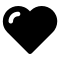
\includegraphics{./images/Een-beetje-verliefd}

\end{column}

\begin{column}{0.34\textwidth}

~

\end{column}

\begin{column}{0.33\textwidth}

\textbf{Een beetje verliefd} \citep{Een-beetje-verliefd} {[}\emph{Trochę zakochany}{]} to piosenka o niespełnionej miłości Rozpoczyna się w scenerii podobnej do tej z piosenki \ref{Leef} wykonanej przez syna André Hazes jr.

\end{column}

\vfill

\begin{column}{0.48\textwidth}

In een discotheek, zat ik van de week\\
En ik voelde mij daar zo alleen\\
't Was er warm en druk, ik zat naast een lege kruk\\
Ik verlangde zo naar jou hier aan m'n zij

\end{column}

\begin{column}{0.04\textwidth}

~

\end{column}

\begin{column}{0.48\textwidth}

W jakiejś dyskotece byłem na tygodniu\\
I czułem się tam bardzo samotny\\
Było tam gorąco i tłoczno, siedziałem przy pustym stołku\\
Tak pragnąłem cię tutaj przy moim boku

\end{column}

\vfill

\begin{column}{0.48\textwidth}

Ja, ik denk nog steeds hoe het was geweest\\
Toen je naast me zat hier aan de bar\\
Ik vroeg: `'Drink je mee?'', dat vond jij oké\\
Toen je proostend naar me keek werd ik zo week

\end{column}

\begin{column}{0.04\textwidth}

~

\end{column}

\begin{column}{0.48\textwidth}

Tak, wciąż się zastanawiam, jak to było\\
Gdy się do mnie przysiadłaś przy barze\\
Spytałem: `'Napijesz się ze mną?'', zgodziłaś się\\
Kiedy na mnie spojrzałaś przy toaście, stałem się taki miękki

\end{column}

\vfill

\begin{column}{0.48\textwidth}

\emph{Een beetje verliefd, ik dacht een beetje verliefd}\\
\emph{Als ik wist wat jij toen dacht, had ik nooit op jou gewacht}\\
\emph{Als een kind zat ik te dromen deze nacht ben jij voor mij}\\
\emph{Maar die droom ging snel voorbij}

\end{column}

\begin{column}{0.04\textwidth}

~

\end{column}

\begin{column}{0.48\textwidth}

\emph{Trochę zakochany, myślałem trochę zakochany}\\
\emph{Gdybym wiedział, co wtedy myślisz, nigdy bym na ciebie nie czekał}\\
\emph{Jak małe dziecko ciągle marzyłem, tej nocy jesteś dla mnie}\\
\emph{Ale ten sen szybko minął}

\end{column}

\vfill

\begin{column}{0.48\textwidth}

Jij stond op en zei: `'Hou m'n plaatsje vrij\\
Ik moet even weg maar ben zo terug''\\
Ach, die kruk bleef leeg tot ik in de gaten kreeg\\
Dat je wegging zonder mij, ik was nu alleen

\end{column}

\begin{column}{0.04\textwidth}

~

\end{column}

\begin{column}{0.48\textwidth}

Wstałaś i powiedziałaś: `'Zajmij mi miejsce\\
Muszę na chwilę wyjść, ale zaraz wrócę''\\
Ach, ten stołek stał pusty, dopóki nie zauważyłem\\
Że odeszłaś beze mnie, teraz byłem sam

\end{column}

\vfill

\begin{itemize}
\tightlist
\item
  \textbf{Weet je wat, ik ben er zat van.} Wiesz co, mam tego dosyć.\\
\item
  \textbf{Ik verlang ernaar met je alleen te zijn.} Pragnę być z tobą sam.\\
\item
  \textbf{Ik heb de wet aan m'n zij(-de).} Prawo mam po swojej stronie.\\
\item
  \textbf{Dat vind ik erg leuk.} To mi się bardzo podoba.\\
\item
  \textbf{We zitten te praten.} Gadamy sobie.\\
\item
  \textbf{Ik krijg dit in de gaten.} Zdaję sobie sprawę z tego
\end{itemize}

\hypertarget{Nacht}{%
\section{\texorpdfstring{Nacht, \emph{Guus Meeuwis and Kraantje Pappie}}{Nacht, Guus Meeuwis and Kraantje Pappie}}\label{Nacht}}

\begin{column}{0.33\textwidth}

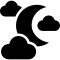
\includegraphics{./images/Nacht}

\end{column}

\begin{column}{0.34\textwidth}

~

\end{column}

\begin{column}{0.33\textwidth}

\textbf{Nacht} \citep{Nacht} {[}\emph{Noc}{]} Ćwierć wieku po Het is een nacht Guus Meeuwis wykonał ``Nacht'' wraz z raperem Kraantje Pappie. Posłuchajcie sami.

\end{column}

\vfill

\begin{column}{0.48\textwidth}

\emph{Het is een nacht}\\
\emph{Die je normaal alleen in films ziet}\\
\emph{Het is een nacht}\\
\emph{Die wordt bezongen in het mooiste lied}\\
\emph{Het is een nacht}\\
\emph{Waarvan ik dacht dat ik hem nooit beleven zou}\\
\emph{Maar vannacht beleef ik hem met jou oh oh}

\end{column}

\begin{column}{0.04\textwidth}

~

\end{column}

\begin{column}{0.48\textwidth}

\emph{To jest taka noc}\\
\emph{Którą widzisz zwykle tylko w filmach}\\
\emph{To jest taka noc}\\
\emph{O której mówi najpiękniejsza piosenka}\\
\emph{To jest taka noc}\\
\emph{O której myślałem, że jej nigdy nie przeżyję}\\
\emph{A którą dziś przeżywam z tobą Ooo}

\end{column}

\vfill

\begin{column}{0.48\textwidth}

Op de grond ligt Châteauneuf-du-Pape\\
De radio zacht, rond middernacht\\
Ik hoor Suus en Freek, een blauwe dag\\
En ik kijk hoe je slaapt, ik hou je vast\\
Want ik weet dat het niet lang meer duurt voor jij gaat\\
Ik snap dat jij me niet te dichtbij laat\\
En je weer vrijmaakt en je op tijd staat\\
Je twijfelt aan of ik wel echt meen wat ik heb gezegd\\
En of ik nog steeds wel de echte ben\\
En of ik niet ren naar 050 en je niet meer ken als een slechte vent\\
Maar vannacht is dat allemaal niet de case\\
Voor nu is het nog nooit zo mooi geweest\\
Jij en ik, the road can wait\\
En ben ik voor eerst opeens compleet

\end{column}

\begin{column}{0.04\textwidth}

~

\end{column}

\begin{column}{0.48\textwidth}

Na ziemi leży Châteauneuf-du-Pape\\
Radio cicho gra, jest koło północy\\
Słyszę Suus i Freek, jakiś niebieski dzień\\
Patrzę jak śpisz, przytulam cię\\
Bo wiem, że to nie potrwa już długo zanim wyjdziesz\\
Rozumiem, że nie pozwolisz mi się zbliżyć\\
En je weer vrijmaakt en je op tijd staat\\
Wątpisz, czy naprawdę mam na myśli to, co powiedziałem\\
I czy nadal jestem prawdziwy\\
I czy nie biegnę na 50 i już cię nie znam jak jakiś zły facet\\
Ale dziś w nocy to w ogóle nie o to chodzi\\
Jeszcze nigdy nie było tak pięknie\\
Ty i ja, droga może poczekać\\
Nagle po raz pierwszy jestem spełniony

\end{column}

\vfill

\begin{column}{0.48\textwidth}

\emph{Als het komt, zou ik steeds met je zijn}\\
\emph{En als je wennen moet, begrijp ik baby, neem je de tijd}\\
\emph{Hier leven we voor, plus cash en baguettes}\\
\emph{En deze nacht heeft alles wat ik zocht op deze plek}

\end{column}

\begin{column}{0.04\textwidth}

~

\end{column}

\begin{column}{0.48\textwidth}

\emph{Gdyby tak się stało, zawsze byłbym z tobą}\\
\emph{A jeśli musisz się zastanowić, rozumiem to baby, nie spiesz się}\\
\emph{Po to żyjemy, plus kasa i bagietki}\\
\emph{I ta noc ma wszystko, co szukałem w tym miejscu}

\end{column}

\vfill

\begin{column}{0.48\textwidth}

Hey schat, ik zou m'n kleine teen geven voor nog één nacht\\
Het is natuurlijk geen wonder dat ik je\\
Donderdag al bijzonder zag in het dons gepakt heb\\
En onze nacht werd er één als\\
Die van Leo en Kate was\\
We on top of the world, ben volledig gebrainwashed\\
But I like it, yeah, jij showt wat life is\\
En ja, je life is er een als Kylie's\\
Maar net iets ronder en iets gezonder\\
Dat is precies hoe mijn vibe is, yeah\\
Jij bent de nicest\\
Bel de Bel, boy, bestel champagne\\
Fuck the prices, je rolt met Crane

\end{column}

\begin{column}{0.04\textwidth}

~

\end{column}

\begin{column}{0.48\textwidth}

Hej kochanie, oddałbym mój mały palec u nogi za jeszcze jedną noc\\
Oczywiście to nic dziwnego, że ja ciebie\\
Donderdag al bijzonder zag in het dons gepakt heb\\
A nasza noc stała się taką jedną,\\
Jaka należała do Leo i Kate\\
Jesteśmy na szczycie świata, mam kompletnie wyprany mózg\\
Ale lubię to, tak, pokazujesz, czym jest życie\\
I tak, twoje życie jest takie jak życie Kylie\\
Ale nieco bardziej zaokrąglone i nieco zdrowsze\\
Dokładnie taki jest mój klimat, tak\\
Jesteś najmilsza\\
Bel de Bel, chłopie, zamówmy szampana\\
Pieprzyć ceny, ty kręcisz z Crane

\end{column}

\vfill

\begin{column}{0.48\textwidth}

Maar vannacht beleef ik 'm met jou, oh\\
Ja ik hou alleen nog maar van jou\\
Ja ik hou alleen nog maar van jou

\end{column}

\begin{column}{0.04\textwidth}

~

\end{column}

\begin{column}{0.48\textwidth}

Ale dziś przeżywam ją z tobą Ooo\\
I kocham tylko wyłącznie ciebie\\
I kocham tylko wyłącznie ciebie

\end{column}

\vfill

\begin{itemize}
\tightlist
\item
  \textbf{Châteauneuf-du-Pape} fr. cenione wino\\
\item
  \textbf{Suus en Freek} duet wykonujący Blauwe Dag \ref{Blauwe-dag}\\
\item
  \textbf{Leo en Kate} para z filmu Titanic\\
\item
  \textbf{Kylie} amerykańska celebrytka\\
\item
  \textbf{Bel de Bel} właść. fr. La Belle des belles\\
\item
  \textbf{Crane} od Kraantje, wykonawcy piosenki
\end{itemize}

\hypertarget{Het-is-een-nacht}{%
\section{\texorpdfstring{Het is een nacht, \emph{Guus Meeuwis}}{Het is een nacht, Guus Meeuwis}}\label{Het-is-een-nacht}}

\begin{column}{0.33\textwidth}

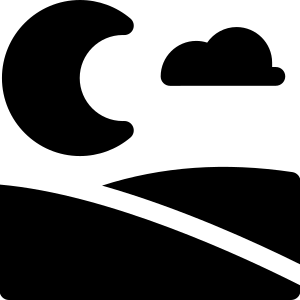
\includegraphics{./images/Het-is-een-nacht}

\end{column}

\begin{column}{0.34\textwidth}

~

\end{column}

\begin{column}{0.33\textwidth}

\textbf{Het is een nacht} \citep{Het-is-een-nacht} {[}\emph{To jest taka noc}{]} powstała po romantycznym weekendzie, jaki spędził autor ze swoją dziewczyną Valérie Gregoire w Brugii.

\end{column}

\vfill

\begin{column}{0.48\textwidth}

Je vraagt of ik zin heb in een sigaret\\
Het is twee uur 's nachts\\
We liggen op bed\\
In een hotel in een stad\\
Waar niemand ons hoort\\
Waar niemand ons kent\\
En niemand ons stoort\\
Op de vloer ligt een lege fles wijn\\
En kledingstukken die van jou of mij kunnen zijn\\
Een schemering de radio zacht\\
En deze nacht heeft alles\\
Wat ik van een nacht verwacht

\end{column}

\begin{column}{0.04\textwidth}

~

\end{column}

\begin{column}{0.48\textwidth}

Pytasz, czy mam ochotę na papierosa\\
Jest druga w nocy\\
Jesteśmy w łóżku\\
W hotelu, w mieście\\
Gdzie nikt nas nie słyszy\\
Gdzie nikt nas nie zna\\
I nikt nam nie przeszkadza\\
Na podłodze leży pusta butelka po winie\\
I ubrania, które mogą być twoje lub moje\\
Półmrok, radio cicho gra\\
I ta noc ma wszystko\\
Czego oczekuję od nocy

\end{column}

\vfill

\begin{column}{0.48\textwidth}

\emph{Het is een nacht}\\
\emph{Die je normaal alleen in films ziet}\\
\emph{Het is een nacht}\\
\emph{Die wordt bezongen in het mooiste lied}\\
\emph{Het is een nacht}\\
\emph{Waarvan ik dacht dat ik hem nooit beleven zou}\\
\emph{Maar vannacht beleef ik hem met jou ohoh}

\end{column}

\begin{column}{0.04\textwidth}

~

\end{column}

\begin{column}{0.48\textwidth}

\emph{To jest taka noc}\\
\emph{Którą widzisz zwykle tylko w filmach}\\
\emph{To jest taka noc}\\
\emph{O której mówi najpiękniejsza piosenka}\\
\emph{To jest taka noc}\\
\emph{O której myślałem, że jej nigdy nie przeżyję}\\
\emph{A którą dziś przeżywam z tobą Ooo\ldots{}}

\end{column}

\vfill

\begin{column}{0.48\textwidth}

Ik ben nog wakker en ik staar naar het plafond\\
En ik denk aan de dag lang geleden begon\\
Het zomaar er vandoor gaan met jou\\
Niet wetend waar de reis eindigen zou\\
Nu lig ik hier in een wildvreemde stad\\
En heb net de nacht van mijn leven gehad\\
Maar helaas er komt weer licht door de ramen\\
Hoewel voor ons de wereld\\
Vannacht heeft stil gestaan

\end{column}

\begin{column}{0.04\textwidth}

~

\end{column}

\begin{column}{0.48\textwidth}

Nadal nie śpię i wpatruję się w sufit\\
I myślę o tym dniu co zaczął się tak dawno\\
Tak po prostu przemija przy tobie\\
Nie wiedząc, gdzie zakończy się ta podróż\\
Teraz leżę tutaj w zupełnie obcym mieście\\
I właśnie miałem noc swojego życia\\
Ale niestety światło znów wpada przez okna\\
Ale co tam, świat dla nas\\
Zatrzymał się dziś w nocy

\end{column}

\vfill

\begin{column}{0.48\textwidth}

Maar een lied blijft slechts bij woorden\\
Een film is in scene gezet\\
Maar deze nacht met jou\\
Is levensecht

\end{column}

\begin{column}{0.04\textwidth}

~

\end{column}

\begin{column}{0.48\textwidth}

Ale piosenka to tylko słowa\\
Film jest udawany\\
Ale dzisiejsza noc z tobą\\
Jest prawdziwa

\end{column}

\vfill

\begin{column}{0.48\textwidth}

En vannacht beleef ik hem met jou ohoh\\
En ik hou alleen nog maar van jou ohoh\\
En ik hou alleen nog maar van jou

\end{column}

\begin{column}{0.04\textwidth}

~

\end{column}

\begin{column}{0.48\textwidth}

I dziś przeżywam ją z tobą Ooo\ldots{}\\
I kocham tylko wyłącznie ciebie Ooo\ldots{}\\
I kocham tylko wyłącznie ciebie

\end{column}

\vfill

\begin{itemize}
\tightlist
\item
  \textbf{Je bent trouwens eigenlijk wel geweldig.} Nawiasem mówiąc, jesteś naprawdę świetny.\\
\item
  \textbf{Als ik niet Pools was, zou ik geen Pools kennen.} Gdybym nie był Polakiem, nie znałbym polskiego.\\
\item
  \textbf{Heb ik daarvoor een vergunning nodig?} Czy potrzebuję na to zezwolenie?\\
\item
  \textbf{Waar kan ik meer te weten komen over \ldots?} Gdzie mogę dowiedzieć się więcej o\ldots?\\
\item
  \textbf{Wanneer \ldots{}} Kiedy \ldots\ldots..?\\
\item
  \textbf{Ik heb zin in een borrel.} Mam ochotę na drinka.\\
\item
  \textbf{De lijn is bezet. Linia jest zajęta}\\
\item
  \textbf{Als ik meer tijd had, zou ik op je wachten.} Gdybym miał/a więcej czasu, poczekałbym na ciebie.\\
\item
  \textbf{Je moeder kan echt lekker koken.} Twoja mama naprawdę potrafi dobrze gotować.\\
\item
  \textbf{Dat is veel, he?} To dużo, prawda?\\
\item
  \textbf{Wanneer moet ik terugkomen?} Kiedy muszę wrócić?\\
\item
  \textbf{Zullen wij naar de duinen gaan?} Może pójdziemy na wydmy?
\end{itemize}

\hypertarget{Blauwe-dag}{%
\section{\texorpdfstring{Blauwe dag, \emph{Suzan \& Freek}}{Blauwe dag, Suzan \& Freek}}\label{Blauwe-dag}}

\begin{column}{0.33\textwidth}

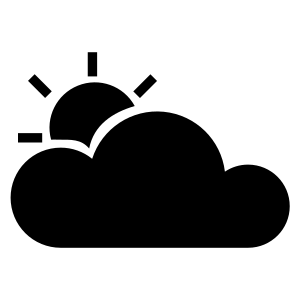
\includegraphics{./images/Blauwe-dag}

\end{column}

\begin{column}{0.34\textwidth}

~

\end{column}

\begin{column}{0.33\textwidth}

\textbf{Blauwe dag} \citep{Blauwe-dag} {[}\emph{Gorszy dzień}{]} powstała po romantycznym weekendzie, jaki spędził autor ze swoją dziewczyną Valérie Gregoire w Brugii.

\end{column}

\vfill

\begin{column}{0.48\textwidth}

Weet je nog dat jij me zei dat wij nooit zouden vluchten als een van ons\\
Loopt door de regen en nooit meer kijkt naar hoe het leven is in de zon\\
Weet je nog dat jij me zei dat jij d'r altijd bent als ik je nodig heb\\
Nee, ik ben het niet vergeten, nee\\
Wat jij me ooit hebt gezegd\\
Want ik zie dat jij het moeilijk hebt en niet meer lachen kan zoals je vroeger deed\\
En nauwelijks in de gaten hebt dat je anders loopt dan dat je deed voorheen\\
Weet je nog dat jij me zei dat jij d'r altijd bent als ik je nodig heb\\
Nee, ik ben het niet vergeten, nee\\
Wat jij me ooit hebt gezegd

\end{column}

\begin{column}{0.04\textwidth}

~

\end{column}

\begin{column}{0.48\textwidth}

Czy pamiętasz, jak mi powiedziałaś, że nigdy nie moglibyśmy uciec, gdyby któreś z nas\\
Szło w deszczu i nie widziało więcej jakie jest życie w słońcu\\
Pamiętasz, jak mi powiedziałeś, że tam zawsze jesteś, kiedy ja cię potrzebuję\\
Nie, ja tego nie zapominałam, nie\\
Co mi kiedyś powiedziałeś\\
Ponieważ widzę, że masz trudności i nie możesz się uśmiechać tak jak kiedyś\\
I prawie nie zauważasz, że chodzisz inaczej niż kiedyś\\
Czy pamiętasz, jak mi powiedziałaś, że tam zawsze jesteś, kiedy ja cię potrzebuję\\
Nie, ja tego nie zapomniałam, nie\\
Co mi kiedyś powiedziałeś

\end{column}

\vfill

\begin{column}{0.48\textwidth}

\emph{Blauwe dag, als het dondert}\\
\emph{En valt de hemel naar beneden, ben ik hier bij jou alleen}\\
\emph{Blauwe dag, een seconde}\\
\emph{Laten we dansen tot de morgen en de lucht weer opengaat}\\
\emph{Fiets met jou mee door heel de stad}\\
\emph{Als jij dat wil, nou, dan doe ik dat}\\
\emph{Ik ben hier op je blauwe dag}\\
\emph{Blauwe dag, een seconde}\\
\emph{Laten we dansen tot de morgen en de lucht weer opengaat}

\end{column}

\begin{column}{0.04\textwidth}

~

\end{column}

\begin{column}{0.48\textwidth}

\emph{Gorszy dzień, kiedy grzmi}\\
\emph{I niebo spada w dół, jestem tu sam przy tobie}\\
\emph{Gorszy dzień, jedna sekunda}\\
\emph{Tańczmy do rana i niebo znów się otwiera}\\
\emph{Jechać z tobą na rowerze przez całe miasto}\\
\emph{Jeśli tego chcesz, teraz, to ja to zrobię}\\
\emph{Jestem tu w twój gorszy dzień}\\
\emph{Gorszy dzień, jedna sekunda}\\
\emph{Przetańczmy tę noc, a niebo znów się przejaśni}

\end{column}

\vfill

\begin{column}{0.48\textwidth}

Weet je nog dat jij me zei dat jij d'r altijd bent wanneer ik ergens val\\
Nu lig ik zelf op de grond en ben ik diegene zonder licht in een donker dal\\
Ik ging van de top van de wereld naar de plek waar ik niemand ken\\
Nee, ik ben het niet vergeten, nee\\
Wat jij me ooit hebt gezegd\\
Blauwe dag, als het dondert\\
En valt de hemel naar beneden, ben ik hier bij jou alleen

\end{column}

\begin{column}{0.04\textwidth}

~

\end{column}

\begin{column}{0.48\textwidth}

Pamiętasz, kiedy powiedziałeś mi, że zawsze tam jesteś, kiedy gdzieś upadam\\
Nu lig ik zelf op de grond en ben ik diegene zonder licht in een donker dal\\
Ik ging van de top van de wereld naar de plek waar ik niemand ken\\
Nee, ik ben het niet vergeten, nee\\
Wat jij me ooit hebt gezegd\\
Blauwe dag, als het dondert\\
En valt de hemel naar beneden, ben ik hier bij jou alleen

\end{column}

\vfill

\begin{column}{0.48\textwidth}

Fiets met jou mee door heel de stad\\
Als jij dat wil, nou, dan doe ik dat\\
Ik ben hier op je blauwe dag\\
Blauwe dag, een seconde\\
Laten we dansen tot de morgen en de lucht weer opengaat

\end{column}

\begin{column}{0.04\textwidth}

~

\end{column}

\begin{column}{0.48\textwidth}

Fiets met jou mee door heel de stad\\
Als jij dat wil, nou, dan doe ik dat\\
Ik ben hier op je blauwe dag\\
Blauwe dag, een seconde\\
Laten we dansen tot de morgen en de lucht weer opengaat

\end{column}

\vfill

\begin{itemize}
\tightlist
\item
  \textbf{De lucht wordt donker.} Niebo robi się ciemne.\\
\item
  \textbf{De lucht klaarde op.} Niebo się przejaśniło.\\
\item
  \textbf{De hemel is blauw} Niebo jest niebieskie.\\
\item
  \textbf{Zijn ziel was in het hemel} Jego dusza była w niebie.\\
\item
  \textbf{Ik voel me blauw.} Jestem przygnębiony.\\
\item
  \textbf{Weet je nog?} Czy pamiętasz?\\
\item
  \textbf{Laten we haar alleen laten.} Zostawmy ją w spokoju.\\
\item
  \textbf{Ik denk dat wij goede vrienden zouden kunnen zijn.} Myślę, że moglibyśmy być dobrymi przyjaciółmi.\\
\item
  \textbf{Hij kan nauwelijks lezen.} On ledwo umie czytać.\\
\item
  \textbf{Houd deze koffer in de gaten.} Obserwuj tę walizkę.
\end{itemize}

\hypertarget{Dromen-zijn-bedrog}{%
\section{\texorpdfstring{Dromen zijn bedrog, \emph{Marco Borsato}}{Dromen zijn bedrog, Marco Borsato}}\label{Dromen-zijn-bedrog}}

\begin{column}{0.33\textwidth}

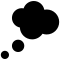
\includegraphics{./images/Dromen-zijn-bedrog}

\end{column}

\begin{column}{0.34\textwidth}

~

\end{column}

\begin{column}{0.33\textwidth}

\textbf{Dromen zijn bedrog} \citep{Dromen-zijn-bedrog} {[}\emph{Sny są ulotne}{]} jest uważana za jeden z najbardziej udanych singli w języku niderlandzkim wszech czasów.

\end{column}

\vfill

\begin{column}{0.48\textwidth}

Steeds als ik je zie lopen dan gaat de hemel een klein beetje open\\
Sterren, je laat ze verbleken met je ogen die altijd stralen\\
Jij kan de zon laten schijnen want je loopt langs en de wolken verdwijnen en als je lacht, lacht heel de wereld mee

\end{column}

\begin{column}{0.04\textwidth}

~

\end{column}

\begin{column}{0.48\textwidth}

Zawsze, kiedy widzę jak idziesz, wtedy odrobinę otwiera się niebo\\
Gwiazdy, sprawiasz że one bledną, swoimi oczami, które cały czas promienieją\\
Możesz pozwolić słońcu świecić, bo gdy przechodzisz chmury znikają a kiedy się śmiejesz, razem śmieje się cały świat

\end{column}

\vfill

\begin{column}{0.48\textwidth}

\emph{De meeste dromen zijn bedrog maar als ik wakker word naast jou dan droom ik nog}\\
\emph{Ik voel je adem en zie je gezicht je bent een droom die naast me ligt}\\
\emph{Je kijkt me aan en rekt je uit een keer in de zoveel tijd komen dromen uit!}

\end{column}

\begin{column}{0.04\textwidth}

~

\end{column}

\begin{column}{0.48\textwidth}

\emph{Najczęściej sny są ulotne, ale kiedy budzę się obok ciebie, wciąż marzę}\\
\emph{Czuję twój oddech i widzę twoją twarz, jesteś snem leżącym obok mnie}\\
\emph{Patrzysz na mnie i się wyciągasz raz na jakiś czas marzenia się spełniają!}

\end{column}

\vfill

\begin{column}{0.48\textwidth}

Jij moet me een ding beloven laat me nog lang in mijn dromen geloven\\
Zelfs als je even niet hier bent blijf in mijn slaap dan bij me\\
En als de zon weer gaat schijnen laat dan dat beeld wat ik heb niet verdwijnen. Als je zou gaan, neem je mijn dromen mee

\end{column}

\begin{column}{0.04\textwidth}

~

\end{column}

\begin{column}{0.48\textwidth}

Musisz mi obiecać jedno, pozwól mi jeszcze długo wierzyć w moje marzenia\\
Nawet jeśli cię chwilę tutaj nie ma, zostań ze mną kiedy śpię\\
A kiedy znów zaświeci słońce, nie pozwól fantazji którą mam zniknąć. Gdybyś szła, zabierz ze sobą moje marzenia

\end{column}

\vfill

\begin{itemize}
\tightlist
\item
  \textbf{Dromen zijn bedrog.} Sen mara, Bóg wiara. {[}prov. za Czochralski{]}\\
\item
  \textbf{Met een klein beetje geluk.} Przy odrobinie szczęścia.\\
\item
  \textbf{De deur gaat niet open, hij klemt.} Drzwi się nie otwierają, są zablokowane.\\
\item
  \textbf{Kom met me mee.} Chodź razem ze mną.\\
\item
  \textbf{Als ik vragen mag.} Jeśli wolno spytać.\\
\item
  \textbf{Ik reik mijn hand naar je uit.} Wyciągam rękę do ciebie.\\
\item
  \textbf{De narcissen kwamen uit.} Wypuściły żonkile.\\
\item
  \textbf{Een keer in de zoveel tijd.} Raz na jakiś czas.\\
\item
  \textbf{Mag ik even binnenkomen?} Czy mogę na chwilę wejść?\\
\item
  \textbf{Ik blijf in slaap vallen.} Ciągle zasypiam.\\
\item
  \textbf{Wat heb je vannacht gedroomd?} Co ci się śniło dzisiaj w nocy?\\
\item
  \textbf{Waar droom je over?} O czym marzysz?
\end{itemize}

\hypertarget{Ik-kan-het-niet-alleen}{%
\section{\texorpdfstring{Ik kan het niet alleen, \emph{De Dijk}}{Ik kan het niet alleen, De Dijk}}\label{Ik-kan-het-niet-alleen}}

\begin{column}{0.33\textwidth}

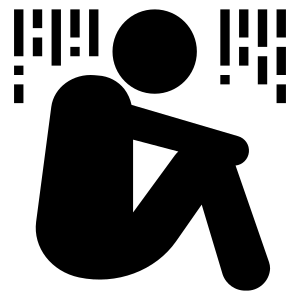
\includegraphics{./images/Ik-kan-het-niet-alleen}

\end{column}

\begin{column}{0.34\textwidth}

~

\end{column}

\begin{column}{0.33\textwidth}

\textbf{Ik kan het niet alleen} \citep{Ik-kan-het-niet-alleen} {[}\emph{Nie mogę tego zrobić sam}{]} to jedna z najbardziej znanych piosenek De Dijk do dziś odtwarzana przez wiele stacji radiowych w Holandii..

\end{column}

\vfill

\begin{column}{0.48\textwidth}

Elke morgen, elke middag\\
Elke avond, iedere nacht\\
Stel dat ik er wel maar jij er niet was\\
Dan was morgen morgen waarschijnlijk weer zo'n dag\\
En ik kan 't niet\\
ik kan 't niet\\
ik kan er niet omheen\\
k-k-kan 't niet\\
ik kan 't niet alleen\\
Natte ramen, kale muren\\
Lege flessen op de gang\\
Lange tanden, late uren\\
Weinig zon en veel behang\\
Ik heb het geprobeerd gedaan wat ik kan\\
maar alles gaat verkeerd\\
Ik ben ook maar een man\\
En ik kan het niet alleen

\end{column}

\begin{column}{0.04\textwidth}

~

\end{column}

\begin{column}{0.48\textwidth}

Co rano, co południe\\
Co wieczór, każdej nocy\\
Stel dat ik er wel maar jij er niet was\\
Jutro prawdopodobnie znowu taki dzień\\
En ik kan 't niet\\
ik kan 't niet\\
ik kan er niet omheen\\
k-k-kan 't niet\\
ik kan 't niet alleen\\
Mokre okna, gołe ściany\\
Puste butelki na korytarzu\\
Brak apetytu Późne godziny\\
Niewiele słońca i wiele tapet\\
Próbowałem zrobić, co mogłem\\
ale wszystko idzie źle\\
Jestem tylko człowiekiem\\
I nie mogę tego zrobić sam

\end{column}

\vfill

\begin{itemize}
\tightlist
\item
  \textbf{Hij eet met lange tanden.} On je niechętnie.\\
\item
  \textbf{Beter laat dan nooit.} Lepiej późno niż wcale.\\
\item
  \textbf{We kunnen er niet omheen dat \ldots{}} Nie możemy omijać faktu, że \ldots{}
\end{itemize}

\hypertarget{O-o-Den-Haag}{%
\section{\texorpdfstring{O, o, Den Haag, \emph{Harry Klorkestein}}{O, o, Den Haag, Harry Klorkestein}}\label{O-o-Den-Haag}}

\begin{column}{0.33\textwidth}

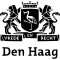
\includegraphics{./images/O-o-Den-Haag}

\end{column}

\begin{column}{0.34\textwidth}

~

\end{column}

\begin{column}{0.33\textwidth}

\textbf{O, o, Den Haag} \citep{O-o-Den-Haag} {[}\emph{Oj, oj, Haga}{]} to piosenka uznawana za nieoficjalny hymn Hagi. Nazwa wykonawcy to anagram nazwy prawdziwego zespołu Klein Orkest.

\end{column}

\vfill

\begin{column}{0.48\textwidth}

Ik zou best nog wel een keertje net als vroeger in Moerwijk willen wonen\\
Na het eten een partijtje voetbal in de tuin, de ouders langs de lijn\\
In december met de hele buurt op jacht om kerstbomen te rausen\\
Op oudejaarsavond fikkie stoken, vooral die autobanden rookten fijn\\
Ik zou best nog wel een keertje met die ouwe naar ADO willen kijken\\
In het Zuiderpark, de lange zij, een warme worst, supporters om je heen\\
Lekker kankeren op Theo van den Burch en die lange van Vianen\\
Want bij elke lage bal dan dook die eikel er steevast overheen\\
O, o, Den Haag, mooie stad achter de duinen\\
De Schilderswijk, de Lange Poten en het Plein\\
O, o, Den Haag, ik zou met niemand willen ruilen\\
Meteen gaan huilen, als ik geen Hagenees zou zijn\\
Ik zou best nog wel een keertje net als vroeger een nachie willen stappen\\
Op mijn Puch een wijffie halen en daarna dansen in de Marathon\\
Na afloop op het Rijswijkseplein een harinkie gaan happen\\
De dag erna een kater dus naar Scheveningen, lekker bakken in de zon\\
Ik zou best nog wel een keertje \ldots{} ach, wat leg ik toch te dromen\\
Want Den Haag is door de jaren zo veranderd, voor mij toch veel te vlug\\
Dat Nieuw Babylon moest dat er trouwens eigenlijk nou wel zo nodig komen?\\
Zo komt die ooievaar op de Vijverberg dus never-nooit meer terug

\end{column}

\begin{column}{0.04\textwidth}

~

\end{column}

\begin{column}{0.48\textwidth}

Bardzo chciałbym raz jeszcze, tak jak kiedyś, na Moerwijku zamieszkać\\
Po obiedzie przyciąć w nogę w ogrodzie, rodzice wzdłuż linii\\
A w grudniu z cała okolica na polowanie co by kilka choinek przyciągnąć\\
W Sylwestra rozniecać pożary, opony dymiły się szczególnie dobrze\\
Bardzo chciałbym raz jeszcze ze starszym na ADO popatrzeć\\
W Zuiderparku, długi bok, ciepła kiełbaska, kibice wokół ciebie\\
Cudne wyzwiska za Theo van den Burch i tym wysokim van Vianen\\
Ponieważ z każdą niska piłka, ten żołądź zawsze przelatywał nad nią\\
O, o, Haga, piękne miasto za wydmami\\
Schilderswijk, Lange Poten no i Plein\\
O, o, Haga, nie chciałbym się z nikim zamienić\\
Płakałbym od razu, gdybym nie był Hażaninem\\
Bardzo chciałbym raz jeszcze, tak jak kiedyś wyjść w noc\\
Zgarnąć laskę na mojego Pucha i potem tańczyć w Marathonie\\
Po wszystkim na Rijswijkseplein pójść śledzika przekąsić\\
Następnego dnia kac, wiec na Scheveningen cudownie smażyć się w słońcu\\
Bardzo chciałbym raz jeszcze \ldots{} ach, o czym ja śnię\\
Ponieważ Haga przez te lata bardzo się zmieniła, jak dla mnie to zbyt szybko\\
Czy ten Nieuw Babylon musiał, tak miedzy nami, się tam pojawić?\\
Wiec nie pojawi się już nigdy więcej bocian na Vijverbergu

\end{column}

\vfill

\begin{itemize}
\tightlist
\item
  \textbf{Ik heb zin in een borrel.} Mam ochotę na drinka.\\
\item
  \textbf{Nog een keer!} Jeszcze raz!\\
\item
  \textbf{Je bent trouwens eigenlijk wel geweldig.} Nawiasem mówiąc, jesteś naprawdę świetny.\\
\item
  \textbf{Als ik niet Pools was, zou ik geen Pools kennen.} Gdybym nie był Polakiem, nie znałbym polskiego.\\
\item
  \textbf{Heb ik daarvoor een vergunning nodig?} Czy potrzebuję na to zezwolenie?\\
\item
  \textbf{Waar kan ik meer te weten komen over \ldots?} Gdzie mogę dowiedzieć się więcej o\ldots?\\
\item
  \textbf{Dat is veel, he?} To dużo, co?\\
\item
  \textbf{Wanneer moet ik terugkomen?} Kiedy muszę wrócić?\\
\item
  \textbf{Zullen wij naar de duinen gaan?} Może pójdziemy na wydmy?\\
\item
  \textbf{De lijn is bezet.} Linia jest zajęta\\
\item
  \textbf{Als ik meer tijd had, zou ik op je wachten.} Gdybym miał/a więcej czasu, poczekałbym na ciebie.\\
\item
  \textbf{Je moeder kan echt lekker koken.} Twoja mama naprawdę potrafi dobrze gotować.
\end{itemize}

\hypertarget{Avond}{%
\section{\texorpdfstring{Avond, \emph{Boudewijn de Groot}}{Avond, Boudewijn de Groot}}\label{Avond}}

\begin{column}{0.33\textwidth}

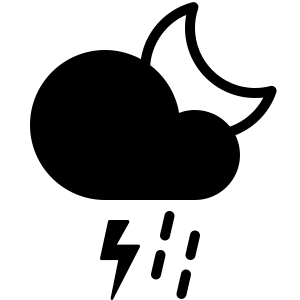
\includegraphics{./images/Avond}

\end{column}

\begin{column}{0.34\textwidth}

~

\end{column}

\begin{column}{0.33\textwidth}

\textbf{Avond} \citep{Avond} {[}\emph{Wieczór}{]} to piosenka uznawana przez Holendrów za najlepszą niderlandzkojęzyczną piosenkę wszechczasóW.

\end{column}

\vfill

\begin{column}{0.48\textwidth}

Nu hoef je nooit je jas meer aan te trekken\\
En te hopen dat je licht het doet\\
Laat buiten de stormwind nu maar razen in het donker\\
Want binnen is het warm en licht en goed\\
Hand in hand naar buiten kijkend waar de regen valt\\
Ik zie het vuur van hoop en twijfel in je ogen\\
En ik ken je diepste angst

\end{column}

\begin{column}{0.04\textwidth}

~

\end{column}

\begin{column}{0.48\textwidth}

Już nie musisz więcej zakładać kurtki\\
I się martwić, czy zapalą światła\\
Niech na dworze w ciemności szaleje wiatr\\
Bo w środku jest ciepło i widno i dobrze\\
Patrząc na dwór, gdzie pada deszcz trzymam cię za rękę\\
W twoich oczach widzę ogień nadziei i zwątpień\\
I znam twój najgłębszy lęk

\end{column}

\vfill

\begin{column}{0.48\textwidth}

\emph{Want je kunt niets zeker weten en alles gaat voorbij}\\
\emph{Maar ik geloof, ik geloof, ik geloof, ik geloof, ik geloof in jou en mij}

\end{column}

\begin{column}{0.04\textwidth}

~

\end{column}

\begin{column}{0.48\textwidth}

\emph{Bo niczego nie możesz być pewna, a wszystko przemija}\\
\emph{Ale wierzę, wierzę, wierzę, wierzę, wierzę w ciebie i we mnie}

\end{column}

\vfill

\begin{column}{0.48\textwidth}

En als je 's morgens opstaat ben ik bij je\\
En misschien heb ik al thee gezet\\
En als de zon schijnt buiten gaan we lopen door de duinen\\
En als het regent gaan we t'rug in bed\\
Uren langzaam wakker worden, zwevend door de tijd\\
Ik zie het licht door de gordijnen\\
En ik weet, t'verleden geeft geen zekerheid

\end{column}

\begin{column}{0.04\textwidth}

~

\end{column}

\begin{column}{0.48\textwidth}

A kiedy wstaniesz rano, to ja będę przy tobie\\
I może herbata już będzie zrobiona\\
I jeśli na dworze będzie słonecznie, to pójdziemy na wydmy\\
A gdyby padało, to wrócimy do łóżka\\
Godziny powoli się budzą unosząc się w czasie\\
Widzę światło przez zasłony\\
I wiem, że przeszłość nie daje pewności

\end{column}

\vfill

\begin{column}{0.48\textwidth}

Ik doe de lichten uit en de kamer wordt nu donker\\
Een straatlantaarn buiten geeft wat licht\\
En de dingen in de kamer worden vrienden die gaan slapen\\
De stoelen staan te wachten op 't ontbijt\\
En morgen wordt ik wakker met de geur van brood en honing\\
De glans van gouden zonlicht in je haar\\
En de dingen in de kamer, ik zeg ze welterusten\\
Vanavond gaan we slapen en morgen zien we wel\\
Maar de dingen in de kamer zouden levenloze dingen zijn\\
Zonder jou

\end{column}

\begin{column}{0.04\textwidth}

~

\end{column}

\begin{column}{0.48\textwidth}

Gaszę światło i teraz w pokoju robi się ciemniej\\
Latarnia na ulicy daje nieco światła\\
A rzeczy w pokoju stają się przyjaciółmi, którzy idą spać\\
Krzesła oczekują na śniadanie\\
A jutro obudzę się z zapachem chleba i miodu\\
Błysk złotych promieni słońca w twoich włosach\\
A rzeczą w pokoju, mówię dobranoc\\
Dzisiaj pójdziemy spać i zobaczymy się znowu jutro\\
Ale rzeczy w pokoju byłyby martwe\\
Bez ciebie

\end{column}

\vfill

\begin{itemize}
\tightlist
\item
  \textbf{Doe het licht maar uit.} Po prostu wyłącz światło.\\
\item
  \textbf{Ik wil je nooit meer zien.} Nie chcę cię nigdy więcej widzieć.\\
\item
  \textbf{Ze liepen hand in hand.} Szli trzymając się za ręce.\\
\item
  \textbf{Die jongen toonde geen angst.} Ten chłopiec nie okazywał strachu.\\
\item
  \textbf{Het is te hopen dat \ldots{}} Należy mieć nadzieją, że \ldots{}\\
\item
  \textbf{De vlam zweeft vaak net boven het hout.} Płomień unosi się często tuż nad drewnem.\\
\item
  \textbf{Ga Maria wakker maken.} Idź obudź Marię\\
\item
  \textbf{Ik sta op het punt uit te gaan.} Zaraz wychodzę.\\
\item
  \textbf{De geur van lelies vulde de kamer.} Zapach lilii wypełnił pokój.\\
\item
  \textbf{De glans wordt gemeten volgens ISO 2813.} Połysk mierzy się zgodnie z ISO 2813.\\
\item
  \textbf{Ik zie je wel bij de auto.} Do zobaczenia w aucie.
\end{itemize}

\hypertarget{Papa}{%
\section{\texorpdfstring{Papa, \emph{Stef Bos}}{Papa, Stef Bos}}\label{Papa}}

\begin{column}{0.33\textwidth}

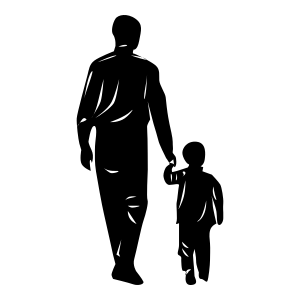
\includegraphics{./images/Papa}

\end{column}

\begin{column}{0.34\textwidth}

~

\end{column}

\begin{column}{0.33\textwidth}

\textbf{Papa} \citep{Papa} {[}\emph{Tato}{]} to wyznanie skierowane do ojca Bosa u którego zdiagnozowano raka. Leczenie Taty się powiodło, zmarł przeżywszy jeszcze 23 lata.

\end{column}

\vfill

\begin{column}{0.48\textwidth}

Ik heb dezelfde ogen\\
En ik krijg jouw trekken om mijn mond\\
Vroeger was ik driftig\\
Vroeger was jij driftig\\
Maar we hebben\\
Onze rust gevonden\\
En we zitten naast elkaar\\
En we zeggen niet zoveel\\
Voor alles wat jij doet\\
Heb ik hetzelfde ritueel\\
Papa, ik lijk steeds meer op jou

\end{column}

\begin{column}{0.04\textwidth}

~

\end{column}

\begin{column}{0.48\textwidth}

Mam oczy takie same\\
A na mojej twarzy rzeźbią się rysy twoje\\
Kiedyś porywczy byłem ja\\
Kiedyś porywczy byłeś ty\\
Ale znaleźliśmy\\
Spokój w sobie\\
I siedzimy obok siebie\\
I mówimy niewiele\\
Do wszystkiego, co robisz\\
Rytuał mam ten sam\\
Tato, coraz bardziej przypominam ciebie

\end{column}

\vfill

\begin{column}{0.48\textwidth}

Ik heb dezelfde handen\\
En ik krijg jouw rimpels in mijn huid\\
Jij hebt jouw ideeën\\
Ik heb mijn ideeën\\
En we zwerven in gedachten\\
Maar we komen altijd thuis\\
De waarheid die je zocht\\
En die je nooit hebt gevonden\\
Ik zoek haar ook\\
En tevergeefs zolang ik leef\\
Want papa, ik lijk steeds meer op jou

\end{column}

\begin{column}{0.04\textwidth}

~

\end{column}

\begin{column}{0.48\textwidth}

Mam ręce takie same\\
A na mojej skórze robią się zmarszczki twoje\\
Ty pomysły masz swoje\\
Ja pomysły mam swoje\\
I wędrujemy w myślach\\
Ale zawsze wracamy z powrotem\\
Ta prawda, której szukałeś\\
I której nigdy nie znalazłeś\\
Też szukam jej ja\\
I na próżno, dopóki żyję\\
Bo tato, coraz bardziej przypominam ciebie

\end{column}

\vfill

\begin{column}{0.48\textwidth}

Vroeger kon je streng zijn\\
En ik heb je soms gehaat\\
Maar jouw woorden\\
Ze liggen op mijn lippen\\
En ik praat nu\\
Zoals jij vroeger praatte\\
Ik heb een goddeloos geloof\\
En ik hou van elke vrouw\\
En misschien ben ik geworden\\
Wat jij helemaal niet wou\\
Maar papa, ik lijk steeds meer op jou

\end{column}

\begin{column}{0.04\textwidth}

~

\end{column}

\begin{column}{0.48\textwidth}

Kiedyś surowy mogłeś być\\
I czasami nienawidziłem ciebie\\
Ale słowa twoje\\
One są na ustach moich\\
A rozmawiam teraz ja\\
Jak rozmawiałeś kiedyś ty\\
Wyznaję bezbożną wiarę\\
I kocham wszystkie kobiety\\
I stałem się może czymś\\
Czego wcale nie chciałeś ty\\
Bo tato, coraz bardziej przypominam ciebie

\end{column}

\vfill

\begin{column}{0.48\textwidth}

Jij gelooft in God\\
Dus jij gaat naar de hemel\\
En ik geloof in niks\\
Dus we komen elkaar na de dood\\
Na de dood nooit meer tegen\\
Maar papa, ik hou steeds meer van jou

\end{column}

\begin{column}{0.04\textwidth}

~

\end{column}

\begin{column}{0.48\textwidth}

Ty wierzysz w Boga\\
Więc pójdziesz do nieba\\
A ja nie wierzę w nic\\
Więc nigdy więcej po śmierci\\
Po śmierci się nie spotkamy\\
Bo tato, coraz bardziej przypominam ciebie

\end{column}

\vfill

\begin{itemize}
\tightlist
\item
  \textbf{Ik zie een kleine glimlach om haar mond trekken.}\\
\item
  \textbf{Ik krijg slaap.} Chce mi się spać.\\
\item
  \textbf{Ik krijg }\\
\item
  \textbf{Niet alles is voor geld te koop.} Nie wszystko można kupić za pieniądze.\\
\item
  \textbf{Ik lijk op mijn moeder.} Wyglądam jak moja matka.\\
\item
  \textbf{Inmiddels ervaren steeds meer mensen de nadelen.} Tymczasem coraz więcej osób doznaje szkód.\\
\item
  \textbf{Ik kom thuis tegen zes uur.} Będę w domu przed szóstą.\\
\item
  \textbf{Hij zwerft al maanden door Europa.} Od miesięcy wędruje po Europie.\\
\item
  \textbf{Zij liggen te praten.} Oni rozmawiają leżąc.\\
\item
  \textbf{Dat ligt mij niet.} To mi nie leży.\\
\item
  \textbf{Eén die weldra op aller lippen zal liggen.} Ten, który wkrótce będzie na ustach wszystkich.
\end{itemize}

\hypertarget{Hij-is-van-mij}{%
\section{\texorpdfstring{Hij is van mij, \emph{Kris Kross Amsterdam x Maan x Tabitha ft. Bizzey }}{Hij is van mij, Kris Kross Amsterdam x Maan x Tabitha ft. Bizzey }}\label{Hij-is-van-mij}}

\begin{column}{0.33\textwidth}

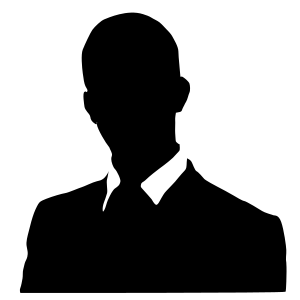
\includegraphics{./images/Hij-is-van-mij}

\end{column}

\begin{column}{0.34\textwidth}

~

\end{column}

\begin{column}{0.33\textwidth}

\textbf{Hij is van mij} \citep{Hij-is-van-mij} {[}\emph{On jest mój}{]} to luźny cover `The Boy Is Mine' amerykańskiego duetu Brenda i Monica. W 2019 roku osiągnął on szczyty holenderskich i flamandzkich list przebojów. to piosenka która nie weszła do listy TOP 2000, ani żaden? wykonawca, ale jest najlepiej sprz się singlem w 2019.

\end{column}

\vfill

\begin{column}{0.48\textwidth}

Voor het eerst in m'n leven\\
Kan ik iemand alles geven\\
Ik voel me veiliger bij je\\
Ja, hij heeft alles wat ik zoek\\
Ik hou `m extra dicht bij me\\
Want al die meiden die kijken\\
Maar hij geeft me geen twijfel

\end{column}

\begin{column}{0.04\textwidth}

~

\end{column}

\begin{column}{0.48\textwidth}

Po raz pierwszy w moim życiu\\
Mogę komuś wszystko dać\\
Przy tobie czuję się bezpieczniej\\
Tak, on ma wszystko, czego szukam\\
Trzymam go bardzo blisko przy sobie\\
Przez te wszystkie dziewczyny, które się patrzą\\
Ale on nie pozwala mi wątpić

\end{column}

\vfill

\begin{column}{0.48\textwidth}

\emph{-Wat ik met hem wil begrijp jij niet}\\
\emph{-Verspil je tijd niet langer, alsjeblieft}\\
\emph{-Jij bent in de war, hij hoort bij mij}\\
\emph{-Dat is niet wat hij zei tegen mij}

\end{column}

\begin{column}{0.04\textwidth}

~

\end{column}

\begin{column}{0.48\textwidth}

\emph{-Nie rozumiesz, czego od niego chcę}\\
\emph{-Nie marnuj więcej czasu, proszę cię}\\
\emph{-Gubisz się, on należy do mnie}\\
\emph{-To nie jest to, co on mi powiedział}

\end{column}

\vfill

\begin{column}{0.48\textwidth}

\emph{Hij is van mij}\\
\emph{Hij zegt dat ik alles voor hem ben}\\
\emph{Dat ik hem het allerbeste ken}\\
\emph{Dat hij aan mij denkt op elk moment}\\
\emph{Hij is van mij}\\
\emph{Het maakt niet uit wat je van mij dacht}\\
\emph{Meisje, weet je niet dat `ie op mij wacht?}\\
\emph{Ik doe hem het beste elke nacht}\\
\emph{Hij is van mij}

\end{column}

\begin{column}{0.04\textwidth}

~

\end{column}

\begin{column}{0.48\textwidth}

\emph{On jest mój}\\
\emph{On mówi, że ja wszystkim dla niego jestem}\\
\emph{Że znam go najlepiej}\\
\emph{Że myli o mnie w każdej chwili}\\
\emph{On jest mój}\\
\emph{To nie ma znaczenia, co o mnie myślisz}\\
\emph{Dziewczyno, czy nie wiesz że on na mnie czeka?}\\
\emph{Robię mu to najlepiej każdej nocy}\\
\emph{On jest mój}

\end{column}

\vfill

\begin{column}{0.48\textwidth}

Hij is het voor mij\\
Geen andere heeft het\\
Hoe hij mij voelt kan niemand beter\\
Hij neemt me voorbij, beter weten\\
Hij heeft m'n naakt, ik zeg het elke dag\\
Ik zeg het elke dag

\end{column}

\begin{column}{0.04\textwidth}

~

\end{column}

\begin{column}{0.48\textwidth}

On jest dla mnie tym\\
Nikt więcej nie ma tego\\
Jak on mnie czuje nie może nikt więcej\\
On bierze mnie na wylot, lepiej wiedzieć\\
On ma moje nagie, mówię że codziennie\\
Mówię że codziennie

\end{column}

\vfill

\begin{column}{0.48\textwidth}

Ey, je zeurt aan m'n hoofd, mama\\
Kijk me in m'n ogen aan\\
Als je mij niet gelooft, mama (Ey, ey, ey)\\
Wat betekent dit dan allemaal?\\
Ik vind het moeilijk om te zeggen hoe het voelt\\
Dat er niks anders is wat is ik mis, nee\\
Jou beschermen, dat is mijn doel\\
Courtois op die bitch, ik mis niks\\
Ik hou van make-up seks, maar dit gaat te ver, uh\\
We don't need to go there (Ooh)\\
You don't wanna go there

\end{column}

\begin{column}{0.04\textwidth}

~

\end{column}

\begin{column}{0.48\textwidth}

Hej, marudzisz mi nad głową, mama\\
Spójrz na mnie w moje oczy\\
Jeśli mi nie wierzysz, mama (Hej, hej, hej)\\
Co zatem znaczy to wszystko?\\
Jest mi trudno powiedzieć, jak się czuję\\
Że nic innego nie ma, co by mi brakowało, nie\\
Bronić cię, to jest mój cel\\
Courtois na tę bitch, mi nie brakuje nic\\
Kocham robić seks, ale to idzie za daleko, uh\\
Nie musimy tam iść (Ooh)\\
Nie chcesz tam iść

\end{column}

\vfill

\begin{column}{0.48\textwidth}

-Maan hij is van mij, oh\\
Niet van jou maar van mij, oh\\
-Tabitha hij is van mij, oh\\
Alleen van mij

\end{column}

\begin{column}{0.04\textwidth}

~

\end{column}

\begin{column}{0.48\textwidth}

-Maan on jest mój, oh\\
Nie twój, ale mój, oh\\
-Tabitha on jest mój, ohoh\\
Tylko mój

\end{column}

\vfill

\begin{itemize}
\tightlist
\item
  \textbf{Kan ik je wat water geven?} Czy mogę ci podać trochę wody?\\
\item
  \textbf{Ik voel me gevleid.} Schlebiasz mi.\\
\item
  \textbf{Ik voel me moe.} Czuję się zmęczony.\\
\item
  \textbf{Ik wil met je meegaan.} Chcę iść z tobą.\\
\item
  \textbf{Ik ben in de war.} Gubię się.\\
\item
  \textbf{Thibaut Nicolas Marc Courtois, belgijski bramkarz} przetłumacz
\end{itemize}

\hypertarget{Het-land-van}{%
\section{\texorpdfstring{Het land van\ldots, \emph{Lange Frans \& Baas B.}}{Het land van\ldots, Lange Frans \& Baas B.}}\label{Het-land-van}}

\begin{column}{0.33\textwidth}


\includegraphics{./images/Het-land-van}

\end{column}

\begin{column}{0.34\textwidth}

~

\end{column}

\begin{column}{0.33\textwidth}

\textbf{Het land van\ldots{}} \citep{Het-land-van} {[}\emph{Kraj pochodzenia}{]} to gniewna litania z wadami i zaletami życia w Holandii. Osobiście zabrakło mi tylko sera, małżeństw jednopłciowych, wiatraków i \ldots{} Polaków.

\end{column}

\vfill

\begin{column}{0.48\textwidth}

Ah \ldots{}\\
Kom uit het land van Pim Fortuyn en Volkert van der G.\\
Het land van Theo van Gogh en Mohammed B.\\
Kom uit het land van kroketten, frikadellen\\
Die je tot aan de Spaanse kust kunt bestellen\\
Kom uit het land waar Air Max nooit uit de mode raken\\
Waar ze je kraken op het moment dat je het groot gaat maken\\
Kom uit het land van rood-wit-blauw en de gouden leeuw

\end{column}

\begin{column}{0.04\textwidth}

~

\end{column}

\begin{column}{0.48\textwidth}

Ach \ldots{}\\
Pochodzę z kraju Pima Fortuin i Volkerta van der G.\\
Z kraju Theo van Gogha i Mohammeda B.\\
Pochodzę z kraju krokietów, frykadeli\\
Które można zamówić aż do wybrzeża Hiszpanii\\
Pochodzą z kraju, w którym Air Max nigdy nie wychodzi z mody\\
W którym cię łamią w momencie, gdy zamierzasz z tego zrobić wielką sprawę\\
Pochodzę z kraju czerwieni, bieli i błękitu oraz złotego lwa

\end{column}

\vfill

\begin{column}{0.48\textwidth}

Plunderen de wereld, dat noemen we de Gouden Eeuw\\
Kom uit het land van wietplantage's en fietsvierdaage's\\
Het land waar je een junkie om een fiets kan vragen\\
Het land dat kampioen werd in `88\\
Het land van haring happen, dijken en grachten\\
Kom uit het land van, het land van Lange Franse\\
Dit is het land waar ik thuis kom na vakantie

\end{column}

\begin{column}{0.04\textwidth}

~

\end{column}

\begin{column}{0.48\textwidth}

Plądrowanie świata, to nazywamy Złotym Wiekiem\\
Pochodzę z kraju plantacji konopi i czterodniowych wycieczek rowerowych\\
Z kraju, w którym możesz poprosić ćpuna o rower\\
Z kraju, który został mistrzem w `88\\
Z kraju, przekąszania śledzia, wałów i kanałów\\
Pochodzę z kraju, kraju Lange Fransa\\
To kraj, do którego wracam do domu z wakacjach

\end{column}

\vfill

\begin{column}{0.48\textwidth}

Ah \ldots{}\\
Kom uit het land waar ik in 1982 geboren ben\\
Waar ik met guldens aan de euro verloren ben\\
Het land dat meedoet aan de oorlog in Irak\\
Want ome Bush heeft Balkenende in zijn zak\\
Het land van gierig zijn, een rondje geven is te duur\\
De vette hap van de `'Febo'' trek je uit de muur\\
Het land van rellen tussen Ajax en Feyenoord

\end{column}

\begin{column}{0.04\textwidth}

~

\end{column}

\begin{column}{0.48\textwidth}

Ach \ldots{}\\
Pochodzę z kraju, w którym się urodziłem w 1982 roku\\
W którym wytraciłem swoje guldeny na euro\\
Z kraju, który bierze udział w wojnie w Iraku\\
Bo wujek Bush ma Balkenende w kieszeni\\
Kraj bycia skąpym, polanie jednej kolejki jest zbyt drogie\\
Tłuste przekąski z „Febo'' wyciągasz ze ściany\\
Kraj zamieszek pomiędzy Ajaxem i Feyenoordem

\end{column}

\vfill

\begin{column}{0.48\textwidth}

Maar wanneer Oranje speelt iedereen erbij hoort\\
Het land van Johan Cruijff en Abe Lenstra\\
Het legioen laat de leeuw niet in zijn hemd staan\\
Het land waar we elke dag hopen op wat beter weer\\
Die Piet Paulusma vertrouw ik voor geen meter meer\\
Het land dat vrij is sinds `45\\
Het land waar ik blijf vind het er heerlijk

\end{column}

\begin{column}{0.04\textwidth}

~

\end{column}

\begin{column}{0.48\textwidth}

Ale kiedy grają pomarańczowi, wszyscy są razem\\
Z kraju Johana Cruijffa i Abe Lenstry\\
Ten legion nie pozwala lwu zostać w samej koszuli\\
Z kraju, w którym każdego dnia mamy nadzieję na lepszą pogodę\\
Temu Pietowi Paulusmie nie wierzę już ani krzty więcej\\
Z kraju, który jest wolny od `45\\
Z kraju, w którym mieszkam, uwielbiam go

\end{column}

\vfill

\begin{column}{0.48\textwidth}

Eerlijk?

\end{column}

\begin{column}{0.04\textwidth}

~

\end{column}

\begin{column}{0.48\textwidth}

Szczerze?

\end{column}

\vfill

\begin{column}{0.48\textwidth}

Ah \ldots{}\\
Kom uit het land waar je door heen rijdt in 3 uurtjes\\
Met een ander dialect elke 10 minuutjes\\
Kom uit het land waar op papier een plek voor iedereen is\\
En XTC, export nummer 1 is\\
Kom uit het land waar André Hazes over 100 jaar in elk café nog steeds de baas is\\
Kom uit het land waar Peter, Gert-Jan, Raymond en Junte, Frans, Bart en Ali de game runnen\\
Kom uit het land waar hiphop een kind van 30 is

\end{column}

\begin{column}{0.04\textwidth}

~

\end{column}

\begin{column}{0.48\textwidth}

Ach \ldots{}\\
Pochodzę z kraju, przez który przejedziesz w 3 godzinki\\
Z innym dialektem co każde 10 minut\\
Pochodzę z kraju, w którym na papierze jest miejsce dla wszystkich\\
A ekstazy to eksportowy numer 1\\
Pochodzę z kraju, w którym André Hazes od stu lat nieustannie każdej kawiarni szefuje\\
Pochodzę z kraju, w którym Peter, Gert-Jan, Raymond oraz Junte, Frans, Bart i Ali prowadzą grę\\
Pochodzę z kraju, w którym Hip-hop jest trzydziestoletnim dzieckiem

\end{column}

\vfill

\begin{column}{0.48\textwidth}

En je mag zelf in gaan vullen hoe vet dat is\\
Het land waar als je rijk wordt je zoveel inlevert\\
En dat je bij jezelf denkt, hoeveel zin heeft het?\\
Het land waar prostitutie en blowen mag\\
Het land van Sinterklaas en Koninginnedag\\
Dit is het land waar ik verloren heb, bedrogen ben\\
Kom uit het land waar ik geboren en getogen ben

\end{column}

\begin{column}{0.04\textwidth}

~

\end{column}

\begin{column}{0.48\textwidth}

Możesz sobie sam wpisać, jakie jest tłuste\\
Z kraju, w którym im bardziej się bogacisz, tym więcej oddajesz\\
I tak się samemu zastanawiasz, ile to ma sensu?\\
Z kraju, w którym prostytucja i palenie trawy są dozwolone\\
Kraj Świętego Mikołaja i Dnia Królowej\\
To jest kraj, w którym coś straciłem, w którym byłem oszukany\\
Pochodzę z kraju, w którym się urodziłem i wychowałem

\end{column}

\vfill

\begin{column}{0.48\textwidth}

Ah \ldots{}\\
Kom uit het land met de meeste culturen per vierkante meter\\
Maar men is bang om bij de buren te gaan eten\\
En `'Integratie'' is een schitterend woord\\
Maar shit is focking bitter wanneer niemand het hoort\\
Ik deel mijn land met Turken en Marokkanen, Antillianen, Molukkers en Surinamers\\
Het land waar we samen veel te veel opkroppen\\
En wereldwijd gerepresenteerd zijn door Harry Potter

\end{column}

\begin{column}{0.04\textwidth}

~

\end{column}

\begin{column}{0.48\textwidth}

Ach \ldots{}\\
Pochodzę z kraju o największej liczbie kultur na metr kwadratowy\\
Ale ludzie boją się jeść u sąsiadów\\
A Integracja to piękne słowo\\
Ale kurwa, aż skręca, że nikt go nie słyszy\\
Dzielę swój kraj z Turkami i Marokańczykami, Antylczykami, Molukami i Surinamczykami\\
Z kraju, w którym o wiele za mocno się razem upychamy\\
I który jest reprezentowany na całym świecie przez Harry'ego Pottera

\end{column}

\vfill

\begin{column}{0.48\textwidth}

Het land waar `'Apartheid''\\
Internationaal het meest bekende woord is uit de Nederlandse taal\\
Kom uit het land dat tikt als een tijdbom\\
Het land dat eet om 6 uur en ook nog eens op tijd komt\\
Dit is het land waar ik zal overwinnen aan het einde\\
Totdat je deze meezingt aan de ArenA lijnen\\
En tot die tijd zal ik schijnen ik heb mijn hart verband

\end{column}

\begin{column}{0.04\textwidth}

~

\end{column}

\begin{column}{0.48\textwidth}

Z kraju, w którym Apartheid\\
Jest na całym świecie najlepiej rozpoznawanym słowem pochodzącym z języka niderlandzkiego\\
Pochodzę z kraju, który tyka jak bomba zegarowa\\
Z kraju, który je o 6 i do tego jeszcze przychodzi się na czas\\
To jest kraj, w którym w końcu zwyciężę\\
Dopóki tego razem ze mną nie zaśpiewasz na trybunach ArenA\\
I do czasu kiedy zabłysnę zabandażowałem moje serce

\end{column}

\vfill

\begin{column}{0.48\textwidth}

Dit is voor Nederland, Baas B Lange Frans

\end{column}

\begin{column}{0.04\textwidth}

~

\end{column}

\begin{column}{0.48\textwidth}

To jest dla Holandii, Baas B \& Lange Frans

\end{column}

\vfill

\begin{itemize}
\tightlist
\item
  \textbf{Pim Fortuyn (Nederlandse politicus) en Theo van Gogh (filmregisseur) en hun respectievelijke moordenaars Volkert van der G. en Mohammed B.} Pim Fortuyn (holenderski polityk) i Theo van Gogh (reżyser) i odpowiednio ich mordercy Volkert van der G. i Mohammed B.\\
\item
  \textbf{Doorzwemmen tot je aan je grens zit.} Płyń, aż osiągniesz swój limit.\\
\item
  \textbf{Mijn vader gaat een wandeling maken in het park.} Mój ojciec idzie na spacer po parku.\\
\item
  \textbf{Het rood-wit-blauw van de vlag van Nederland.} Kolory czerwono, biały i niebieski na fladze Holandii.\\
\item
  \textbf{De gouden leeuw van het wapen van het Koninkrijk der Nederlanden.} Złoty lew z herbu Królestwa Niderlandów.\\
\item
  \textbf{Lange Frans en Baas B schreef dit nummer.} Lange Frans, Baas B schreef dit nummer.\\
\item
  \textbf{Jan Peter Balkenende is de voormalige premier van Nederland.} Jan Peter Balkenende jest byłym premierem Holandii.\\
\item
  \textbf{Het maakt niet uit.} To nie ma znaczenia.\\
\item
  \textbf{Dit hele ding is gewoon helemaal gek.} Cała ta sprawa jest po prostu zupełnie szalona.\\
\item
  \textbf{Hij zal morgen toch wel weer gaan drinken.} W każdym razie jutro będzie pił znowu.\\
\item
  \textbf{`'Ajax'' en `'Feyenoord'' zijn Nederlandse profvoetbalclubs, terwijl `'Oranje'' het Nederlands voetbalelftal is.} „Ajax'' i „Feyenoord'' to holenderskie profesjonalne kluby piłkarskie, a „Oranje'' to holenderska drużyna narodowa.\\
\item
  \textbf{Ze horen bij mij.} Oni są ze mną.\\
\item
  \textbf{Bekende Nederlandse voetballers zijn Johan Cruijff (met rugnummer 14) en Abe Lenstra.} Znani holenderscy piłkarze to Johan Cruijff (z koszulką nr 14) i Abe Lenstra.\\
\item
  \textbf{Piet Paulusma is een Nederlandse weerman.} Piet Paulusma to holenderski prezenter pogody.\\
\item
  \textbf{Ik haat je nog steeds.} Nadal cię nienawidzę.\\
\item
  \textbf{André Hazes was een populaire Nederlandse zanger.} André Hazes był popularnym holenderskim piosenkarzem. \ref{Een-beetje-verliefd}\\
\item
  \textbf{Peter, Gert-Jan, Raymond, Junte, Frans, Bart en Ali zijn de namen van Nederlandse rappers: Delic, Brainpower, Kid Ray, Sticky Steez, Lange Frans, Baas B en Ali B.} Peter, Gert-Jan, Raymond, Junte, Frans, Bart i Ali to imiona holenderskich raperów: Delic, Brainpower, Kid Ray, Sticky Steez, Lange Frans, Baas B i Ali B.\\
\item
  \textbf{Invullen in hoofdletters} Wpisz wielkimi literami.\\
\item
  \textbf{Ik heb/ben mijn portemonnee verloren.} Zgubiłem portfel.\\
\item
  \textbf{Ik ben bedrogen door jou,} Zostałem przez ciebie oszukany.\\
\item
  \textbf{Het heeft geen zin om zo'n smoes te gebruiken.} Nie ma sensu używać takiej wymówki.\\
\item
  \textbf{Ik had veel te veel gedronken.} Wypiłem dużo za dużo.\\
\item
  \textbf{Moet ze haar emoties dan opkroppen?} Czy powinna zatem zebrać swoje emocje?\\
\item
  \textbf{J. C. M. van Riemsdijk (Nederlandse muzikant en schrijver) is een authentiek personage uit de Harry Potter-films.}J. C. M. van Riemsdijk (holenderski muzyk i pisarz) to autentyczna postać z filmów o Harrym Potterze.
\end{itemize}

\hypertarget{Het-dorp}{%
\section{\texorpdfstring{Het dorp, \emph{Wim Sonneveld}}{Het dorp, Wim Sonneveld}}\label{Het-dorp}}

\begin{column}{0.33\textwidth}

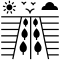
\includegraphics{./images/Het-dorp}

\end{column}

\begin{column}{0.34\textwidth}

~

\end{column}

\begin{column}{0.33\textwidth}

\textbf{Het dorp} \citep{Het-dorp} {[}\emph{Wieś}{]} to wspomnienia autora tekstu o utraconym dzieciństwie. Hugo Verhage to naprawdę Friso Wiegersma. Z wykonawcą piosenki Wimem Sonneveld byli w związku. .

\end{column}

\vfill

\begin{column}{0.48\textwidth}

Thuis heb ik nog een ansichtkaart\\
Waarop een kerk een kar met paard\\
Een slagerij J. van der Ven\\
Een kroeg, een juffrouw op de fiets

\end{column}

\begin{column}{0.04\textwidth}

~

\end{column}

\begin{column}{0.48\textwidth}

W domu wciąż mam pocztówkę\\
Na niej kościół i koń z wozem\\
Sklep mięsny J. van der Ven\\
Pub, nauczycielka na rowerze

\end{column}

\vfill

\begin{column}{0.48\textwidth}

Het zegt u hoogstwaarschijnlijk niets\\
Maar het is waar ik geboren ben\\
Dit dorp, ik weet nog hoe het was\\
De boerenkind'ren in de klas

\end{column}

\begin{column}{0.04\textwidth}

~

\end{column}

\begin{column}{0.48\textwidth}

Pewnie nic ci to nie mówi\\
Ale tam się urodziłem\\
Ta wieś, wciąż pamiętam jak to było\\
Wiejskie dzieci w klasie

\end{column}

\vfill

\begin{column}{0.48\textwidth}

Een kar die ratelt op de keien\\
Het raadhuis met een pomp ervoor\\
Een zandweg tussen koren door\\
Het vee, de boerderijen

\end{column}

\begin{column}{0.04\textwidth}

~

\end{column}

\begin{column}{0.48\textwidth}

Wóz klekocze na kamieniach\\
Ratusz z pompą przed nim\\
Polna droga wśród pszenicy hen\\
Żywy inwentarz, zagrody chłopskie

\end{column}

\vfill

\begin{column}{0.48\textwidth}

\emph{En langs het tuinpad van m'n vader}\\
\emph{Zag ik de hoge bomen staan}\\
\emph{Ik was een kind en wist niet beter}\\
\emph{Dan dat 't nooit voorbij zou gaan}

\end{column}

\begin{column}{0.04\textwidth}

~

\end{column}

\begin{column}{0.48\textwidth}

\emph{I wzdłuż ścieżki w ogrodzie ojca}\\
\emph{Widziałem jak rosną wysokie drzewa}\\
\emph{Byłem dzieckiem i wiedziałem na pewno}\\
\emph{Że to nigdy nie przeminie}

\end{column}

\vfill

\begin{column}{0.48\textwidth}

Wat leefden ze eenvoudig toen\\
In simp'le huizen tussen groen\\
Met boerenbloemen en een heg\\
Maar blijkbaar leefden ze verkeerd

\end{column}

\begin{column}{0.04\textwidth}

~

\end{column}

\begin{column}{0.48\textwidth}

Jakże wtedy żyli zwyczajnie\\
W prostych domach wśród zieleni\\
Z polnymi/wiejskimi kwiatami i żywopłotem\\
Ale widocznie żyli niewłaściwie

\end{column}

\vfill

\begin{column}{0.48\textwidth}

Het dorp is gemoderniseerd\\
En nou zijn ze op de goeie weg\\
Want ziet, hoe rijk het leven is\\
Ze zien de televisiequiz

\end{column}

\begin{column}{0.04\textwidth}

~

\end{column}

\begin{column}{0.48\textwidth}

Wieś została zmodernizowana\\
A teraz są na dobrej drodze\\
Zobacz, jakie życie jest bogate\\
Oglądają teleturniej

\end{column}

\vfill

\begin{column}{0.48\textwidth}

En wonen in betonnen dozen\\
Met flink veel glas, dan kun je zien\\
Hoe of het bankstel staat bij Mien\\
En d'r dressoir met plastic rozen

\end{column}

\begin{column}{0.04\textwidth}

~

\end{column}

\begin{column}{0.48\textwidth}

I mieszkają w betonowych pudełkach\\
Z dużą ilością szkła, wtedy możesz zobaczyć\\
Czy u Mien dobrze stoi kanapa\\
I jej komoda z plastikowymi różami

\end{column}

\vfill

\begin{column}{0.48\textwidth}

\emph{En langs het tuinpad van m'n vader}\\
\emph{Zag ik de hoge bomen staan}\\
\emph{Ik was een kind en wist niet beter}\\
\emph{Dan dat 't nooit voorbij zou gaan}

\end{column}

\begin{column}{0.04\textwidth}

~

\end{column}

\begin{column}{0.48\textwidth}

\emph{I wzdłuż ścieżki w ogrodzie ojca}\\
\emph{Widziałem jak rosną wysokie drzewa}\\
\emph{Byłem dzieckiem i wiedziałem na pewno}\\
\emph{Że to nigdy nie przeminie}

\end{column}

\vfill

\begin{column}{0.48\textwidth}

De dorpsjeugd klit wat bij elkaar\\
In minirok en beatle-haar\\
En joelt wat mee met beat-muziek\\
Ik weet wel het is hun goeie recht

\end{column}

\begin{column}{0.04\textwidth}

~

\end{column}

\begin{column}{0.48\textwidth}

Młodzież ze wsi włóczy się razem\\
W spódniczce mini i włosach na Beatlesa\\
I wydzierają się razem przy ich muzyce\\
Wiem dobrze, takie ich święto prawo

\end{column}

\vfill

\begin{column}{0.48\textwidth}

De nieuwe tijd, net wat u zegt\\
Maar het maakt me wat melancholiek\\
Ik heb hun vaders nog gekend\\
Ze kochten zoethout voor een cent

\end{column}

\begin{column}{0.04\textwidth}

~

\end{column}

\begin{column}{0.48\textwidth}

Nowe czasy, co na to poradzisz\\
Ale popadam przy tym w melancholię\\
Już znałem ich ojców\\
Kupili lukrecję za grosz

\end{column}

\vfill

\begin{column}{0.48\textwidth}

Ik zag hun moeders touwtjespringen\\
Dat dorp van toen, het is voorbij\\
Dit is al wat er bleef voor mij\\
Een ansicht en herinneringen

\end{column}

\begin{column}{0.04\textwidth}

~

\end{column}

\begin{column}{0.48\textwidth}

Widziałem ich matki na skakance\\
Tamtej wsi już nie ma\\
To wszystko, co mi pozostało\\
Pocztówka i wspomnienia

\end{column}

\vfill

\begin{column}{0.48\textwidth}

\emph{Toen ik langs het tuinpad van m'n vader}\\
\emph{De hoge bomen nog zag staan}\\
\emph{Ik was een kind, hoe kon ik weten}\\
\emph{Dat dat voorgoed voorbij zou gaan}

\end{column}

\begin{column}{0.04\textwidth}

~

\end{column}

\begin{column}{0.48\textwidth}

\emph{Kiedyś wzdłuż ścieżki w ogrodzie ojca}\\
\emph{Widziałem jak jeszcze rosły wysokie drzewa}\\
\emph{Byłem dzieckiem, skąd mogłem wiedzieć}\\
\emph{Że to na dobre przeminie}

\end{column}

\vfill

\begin{itemize}
\tightlist
\item
  \textbf{Weet je nog?} Czy pamiętasz?\\
\item
  \textbf{Ik weet het nog niet.} Nadal nie wiem.\\
\item
  \textbf{Ik zou graag naar Polen gaan.} Chciałbym pojechać do Polski.\\
\item
  \textbf{Zij gaan totaal voorbij aan het risico.} Całkowicie ignorują ryzyko.\\
\item
  \textbf{Ik heb nog niet gegeten.} Jeszcze nic nie jadłem.\\
\item
  \textbf{Mien is een vorm van Wilhelmina.} Mien jest formą Wilhelminy.
\end{itemize}

\hypertarget{Mag-ik-dan-bij-jou}{%
\section{\texorpdfstring{Mag ik dan bij jou, \emph{Claudia de Breij}}{Mag ik dan bij jou, Claudia de Breij}}\label{Mag-ik-dan-bij-jou}}

\begin{column}{0.33\textwidth}

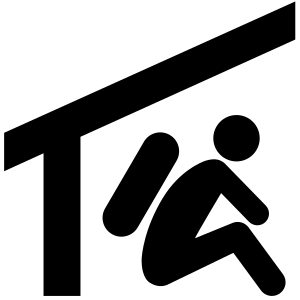
\includegraphics{./images/Mag-ik-dan-bij-jou}

\end{column}

\begin{column}{0.34\textwidth}

~

\end{column}

\begin{column}{0.33\textwidth}

\textbf{Mag ik dan bij jou} \citep{Mag-ik-dan-bij-jou} {[}\_ TITLE.PL\_{]} ??? .

\end{column}

\vfill

\begin{column}{0.48\textwidth}

Als de oorlog komt en als ik dan moet schuilen\\
Mag ik dan bij jou?\\
Als er een clubje komt waar ik niet bij wil horen\\
Mag ik dan bij jou?

\end{column}

\begin{column}{0.04\textwidth}

~

\end{column}

\begin{column}{0.48\textwidth}

Gdy wybuchnie wojna, a ja będę musiała się ukryć\\
Czy będę mogła u ciebie?\\
Gdy powstanie klub, w którym nie chcę być\\
Czy będę mogła u ciebie?

\end{column}

\vfill

\begin{column}{0.48\textwidth}

Als er een regel komt waar ik niet aan voldoen kan\\
Mag ik dan bij jou?\\
En als ik iets moet zijn wat ik nooit geweest ben\\
Mag ik dan bij jou?

\end{column}

\begin{column}{0.04\textwidth}

~

\end{column}

\begin{column}{0.48\textwidth}

Gdy wejdzie reguła, której nie mogę spełnić\\
Czy będę mogła u ciebie?\\
Gdy stanę się kimś, kim nigdy nie byłam\\
Czy będę mogła u ciebie?

\end{column}

\vfill

\begin{column}{0.48\textwidth}

\emph{Mag ik dan bij jou schuilen als het nergens anders kan?}\\
\emph{En als ik moet huilen droog jij m'n tranen dan?}\\
\emph{Want als ik bij jou mag, mag jij altijd bij mij}\\
\emph{Kom wanneer je wilt ik hou een kamer voor je vrij}

\end{column}

\begin{column}{0.04\textwidth}

~

\end{column}

\begin{column}{0.48\textwidth}

\emph{Czy będę mogła u ciebie się schronić, gdy nie będzie gdzie indziej?}\\
\emph{Gdy zapłaczę, czy wysuszysz me łzy?}\\
\emph{Bo jeśli mogę u ciebie, ty zawsze możesz u mnie}\\
\emph{Przyjdź kiedy tylko chcesz, mam dla ciebie wolny pokój}

\end{column}

\vfill

\begin{column}{0.48\textwidth}

Als het onweer komt en als ik dan bang ben\\
Mag ik dan bij jou?\\
Als de avond valt en 't is mij te donker\\
Mag ik dan bij jou?

\end{column}

\begin{column}{0.04\textwidth}

~

\end{column}

\begin{column}{0.48\textwidth}

Gdy zacznie się burza, a ja będę się bała\\
Czy będę mogła u ciebie?\\
Gdy zapadnie wieczór, a mi jest za ciemno\\
Czy będę mogła u ciebie?

\end{column}

\vfill

\begin{column}{0.48\textwidth}

Als de lente komt en als ik dan verliefd ben\\
Mag ik dan bij jou?\\
Als de liefde komt en ik weet het zeker\\
Mag ik dan bij jou?

\end{column}

\begin{column}{0.04\textwidth}

~

\end{column}

\begin{column}{0.48\textwidth}

Gdy zacznie się wiosna, a ja się zakocham\\
Czy będę mogła u ciebie?\\
Gdy przyjdzie miłość, a ja będę tego pewna\\
Czy będę mogła u ciebie?

\end{column}

\vfill

\begin{column}{0.48\textwidth}

Als het einde komt en als ik dan bang ben\\
Mag ik dan bij jou?\\
Als het einde komt en als ik dan alleen ben\\
Mag ik dan bij jou?

\end{column}

\begin{column}{0.04\textwidth}

~

\end{column}

\begin{column}{0.48\textwidth}

Gdy nadejdzie koniec, a ja będę się bała\\
Czy będę mogła u ciebie?\\
Gdy nadejdzie koniec, a ja będę sama\\
Czy będę mogła u ciebie?

\end{column}

\vfill

\begin{itemize}
\tightlist
\item
  \textbf{Mogen we bij jou overnachten?} Czy możemy u ciebie przenocować?\\
\item
  \textbf{De spullen moeten wel aan één regel voldoen.} Przedmioty muszą być zgodne z jedną zasadą.\\
\item
  \textbf{Dat is jouw thuis, daar en nergens anders.} To jest twój dom, tam i nigdzie indziej.\\
\item
  \textbf{Als je niets te zeggen hebt, zeg dan niets.} Jeśli nie masz nic do powiedzenia, nie mów nic.
\end{itemize}

\hypertarget{Pastorale}{%
\section{\texorpdfstring{Pastorale, \emph{Ramses Shaffy \& Liesbeth List}}{Pastorale, Ramses Shaffy \& Liesbeth List}}\label{Pastorale}}

\begin{column}{0.33\textwidth}

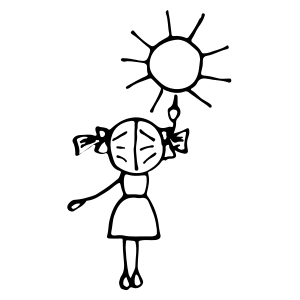
\includegraphics{./images/Pastorale}

\end{column}

\begin{column}{0.34\textwidth}

~

\end{column}

\begin{column}{0.33\textwidth}

\textbf{Pastorale} \citep{Pastorale} {[}\emph{Pastorałka}{]} to psychodeliczna rozmowa ziemskiego dziecka z potężnym słońcem .

\end{column}

\vfill

\begin{column}{0.48\textwidth}

Mijn hemel blauw met gouden hallen, mijn wolkentorens, ijskristallen, kometen, manen en planeten, ah\\
Alles draait om mij

\end{column}

\begin{column}{0.04\textwidth}

~

\end{column}

\begin{column}{0.48\textwidth}

Moje niebo niebieskie ze złotymi salami, moje chmurne wieże, kryształy lodu, komety, księżyce i planety, ach\\
Wszystko się kręci wokół mnie

\end{column}

\vfill

\begin{column}{0.48\textwidth}

En door de witte wolkenpoort tot diep onder de golven boort mijn vuur, mijn liefde, zich in de aarde\\
En bij het water speelt een kind en alle schelpen die het vindt gaan blinken als ik lach

\end{column}

\begin{column}{0.04\textwidth}

~

\end{column}

\begin{column}{0.48\textwidth}

I przez białe chmurne wrota sięgające głębin poniżej fal wkręca się mój ogień, moja miłość, w ziemię\\
A nad wodą bawi się dziecko i wszystkie znalezione przez nie muszle zaczynają błyszczeć gdy się uśmiecham

\end{column}

\vfill

\begin{column}{0.48\textwidth}

\emph{'k Hou van je warmte op mijn gezicht, ik hou van de koperen kleur van je licht}\\
\emph{Ik geef je water in mijn hand en schelpen uit het zoute zand}\\
\emph{Ik heb je lief, zo lief}

\end{column}

\begin{column}{0.04\textwidth}

~

\end{column}

\begin{column}{0.48\textwidth}

\emph{Uwielbiam twoje ciepło na mojej twarzy, uwielbiam miedziany kolor twojego światła}\\
\emph{Daję ci wodę w mojej dłoni i muszle wyjęte ze słonego piasku}\\
\emph{Kocham cię, tak bardzo}

\end{column}

\vfill

\begin{column}{0.48\textwidth}

Ik scheur de rotsen met mijn stralen verhoog de meren in de dalen en onweersluchten doe ik vluchten, ah\\
Als de regen valt

\end{column}

\begin{column}{0.04\textwidth}

~

\end{column}

\begin{column}{0.48\textwidth}

Rozdzieram skały swymi promieniami podnoszę jeziora w dolinach i przeganiam burze, ach\\
Gdy pada deszcz

\end{column}

\vfill

\begin{column}{0.48\textwidth}

Verberg je ogen in mijn hand voordat m'n glimlach ze verbrandt m'n vuur, m'n liefde, mijn gouden ogen\\
't Is beter als je nog wat wacht want even later komt de nacht en schijnt de koele maan

\end{column}

\begin{column}{0.04\textwidth}

~

\end{column}

\begin{column}{0.48\textwidth}

Ukryj swe oczy w mojej dłoni, zanim mój uśmiech je wypali, mój ogień, moja miłość, moje złote oczy\\
Będzie lepiej jak trochę poczekasz, bo nieco później przyjdzie noc i zaświeci chłodny księżyc

\end{column}

\vfill

\begin{column}{0.48\textwidth}

\emph{De nacht is te koud, de maan te grijs toe neem me toch mee naar je hemelpaleis}\\
\emph{Daar wil ik zijn alleen met jou en stralen in het hemelblauw}\\
\emph{Ik heb je lief, zo lief}

\end{column}

\begin{column}{0.04\textwidth}

~

\end{column}

\begin{column}{0.48\textwidth}

\emph{Noc jest zbyt zimna, księżyc zbyt blady, więc zabierz mnie już do twojego niebiańskiego pałacu}\\
\emph{Chcę być tam z tobą sam na sam i promieniować w niebiańskim błękicie}\\
\emph{Kocham cię, tak bardzo}

\end{column}

\vfill

\begin{column}{0.48\textwidth}

Als ik de aarde ga verwarmen laat ik haar leven in m'n armen, van sterren weefde ik het verre, ah\\
Het noorderlicht

\end{column}

\begin{column}{0.04\textwidth}

~

\end{column}

\begin{column}{0.48\textwidth}

Gdy ogrzeję ziemię, pozwolę jej żyć w moich ramionach, z dala od gwiazd utkałem, ach\\
Zorzę polarną

\end{column}

\vfill

\begin{column}{0.48\textwidth}

Maar soms ben ik als kokend lood, ik ben het leven en de dood, in vuur, in liefde, in alle tijden\\
M'n kind ik troost je, kijk omhoog vandaag span ik mijn regenboog die is alleen voor jou

\end{column}

\begin{column}{0.04\textwidth}

~

\end{column}

\begin{column}{0.48\textwidth}

Ale czasami jestem jak wrzący ołów, jestem życiem i śmiercią, w ogniu, w miłości, przez cały czas\\
Moje dziecko, pocieszę cię, spójrz w górę, dziś rozciągam tęczę tylko dla ciebie

\end{column}

\vfill

\begin{column}{0.48\textwidth}

Nee, nooit sta ik een seconde stil, geen mens kan mij dwingen wanneer ik niet wil\\
Geen leven dat ik niet begon, je kunt niet houden van de zon

\end{column}

\begin{column}{0.04\textwidth}

~

\end{column}

\begin{column}{0.48\textwidth}

Nie, nigdy się nie zatrzymam nawet na chwilę, gdy nie chcę, żaden człowiek nie może mnie zmusić\\
Żadne życie, którego nie począłem, nie możesz kochać słońca

\end{column}

\vfill

\begin{column}{0.48\textwidth}

\emph{'k Wil liever branden, neem me mee wanneer je vanavond gaat slapen in zee en vliegen langs jouw hemelbaan}\\
\emph{Ik wil niet meer bij jou vandaan}\\
\emph{Ik heb je lief, zo lief}

\end{column}

\begin{column}{0.04\textwidth}

~

\end{column}

\begin{column}{0.48\textwidth}

\emph{Wolę spłonąć, zabierz mnie ze sobą, gdy wieczorem położysz się spać w morzu i odlecisz po niebiańskiej orbicie}\\
\emph{Nie chcę być dłużej z dala od ciebie}\\
\emph{Kocham cię, tak bardzo}

\end{column}

\vfill

\begin{itemize}
\tightlist
\item
  \textbf{Wie zwijgt, stemt toe.} Milczenie oznacza zgodę.\\
\item
  \textbf{Alsjeblieft, ik wil liever alleen zijn.}Proszę, wolę być sam.\\
\item
  \textbf{Ik heb je lief, ik heb je kinderen lief en je kinderen houden van jou! Kocham cię, kocham twoje dzieci, a twoje dzieci kochają ciebie.}\\
\item
  \textbf{Hij houdt mij niet bij jou vandaan.} Nie zatrzyma mnie z dala od ciebie.
\end{itemize}

\hypertarget{podziemie}{%
\chapter{PODZIEMIE}\label{podziemie}}

\hypertarget{lata-1990---1999}{%
\chapter{Lata 1990 - 1999}\label{lata-1990---1999}}

Miejsce na rozdział

\hypertarget{lata-2000---2009}{%
\chapter{Lata 2000 - 2009}\label{lata-2000---2009}}

Miejsce na rozdział

\hypertarget{lata-2010---2019}{%
\chapter{Lata 2010 - 2019}\label{lata-2010---2019}}

Miejsce na rodział

  \bibliography{songs.bib}

\end{document}
